
\section{Formulation}

\newcommand{\DD}{\mathbf{D}}
\newcommand{\dd}{\mathbf{d}}

We begin by looking at a Light Curtain only problem of adaptively discovering the depth of a scene. We wouldn't know the path along the rays/pixels on which an object may lie/intersect, hence we choose to go with a sampling based approach. We treat each ray as initially having either a uniform distribution, or a gaussian with a large variance in the center, and we attempt to formulate our problem with a Recursive Bayesian update approach.

\subsection{Representation}

\smallskip
We wish to estimate the depth map $\DD = \{d_{u, v}\}$ of the scene, which specifies the depth value $d_{u, v}$ for every camera pixel $(u, v)$. This is represented as a tensor of some fixed resolution [320x240] with each pixel in image $\DD$ encoding the depth value $d_{u,v}$. Since there is inherent uncertainty in the depth value at every pixel, we output a \textit{probability distribution} over depths for every pixel. Let us define $\dd_{u,v}$ to be a \textit{random variable} for depth predictions at the pixel $(u, v)$. We quantize depth values into a set $\D = \{d_0, \dots, d_{N-1}\}$ of $N$ discrete, uniformly spaced depth values lying in $(d_\text{min}, d_\text{max})$. All our predictions $\dd_{u, v} \in \D$ belong to this set. The output of our depth estimation method for each pixel is a probability distribution $P(\dd_{u, v})$, modeled as a categorical distribution over $\D$. In this work, we use $N=64$, resulting in a Depth Probability Volume (DPV) tensor of size [64, 240, 320]
\begin{align}
   &\D=\{d_0, \dots, d_{N-1}\}; d_{q}=d_\text{min}+(d_\text{max}-d_\text{min}) \cdot q
   \label{eq:d_candi}
   \\
   &\sum_{q=0}^{N-1} P(\dd_{u,v} = d_q) =1 \ \text{(q is the quantization index)}
   % \qquad \mathbb{E}[P(\mathbf{d}(u,v))]=\mathbf{d}(u,v)
   \label{eq:depth_dist}\\
   &\text{Depth estimate } = \mathbb{E} [ \dd_{u,v}] = \sum_{q=0}^{N-1} P(\dd_{u,v}=d_q)\cdot d_q
   %\vspace{-.1in}
\end{align}

While an ideal sensor could choose to plan a path to sample in the full 3D volume, our Light Curtain device only has control over a collapsed XZ  space. Hence, we generate an ``Uncertainty Field" (UF) \cite{yang2019inferring}, by avergaing the probabilities of the DPV across columns. While computing this field, we only consider those pixels whose corresponding 3D heights are between $(h_\text{min}, h_\text{max})$. The UF is defined for the camera column $u$ and quantized depth location $q$ as:
\begin{align}
   UF(u, q) =\ &\frac{1}{|\mathcal{V}(u)|}\sum_{v \in \mathcal{V}(u)} P(\dd_{u, v} = d_q)\nonumber\\
   \text{where } &\mathcal{V}(u) = \{v\ |\ h_\text{min} \leq h(u, v) \leq h_\text{max}\} 
   % P(\mathbf{d}(u))=\frac{\sum_{u,v}P(\mathbf{d}{(u,v)}).\boldsymbol{1}}{\sum_{u,v}\boldsymbol{1}}
   % \;where\;h_{min}>\mathbb{E}[P(\mathbf{d}(u,v))]>h_{max}
   \label{eq:collapse}
   %\vspace{-.1in}
\end{align}

We denote the categorical distribution of the uncertainty field on the $u$-th camera ray as \\$UF(u)=\text{Categorical}(d_q \in \D\ |\ P=\{UF(u, q)\}_{q=0}^{N-1}\})$. 

\begin{figure}[h]
   \centering
   \begin{minipage}{0.5\textwidth}
       \centering
       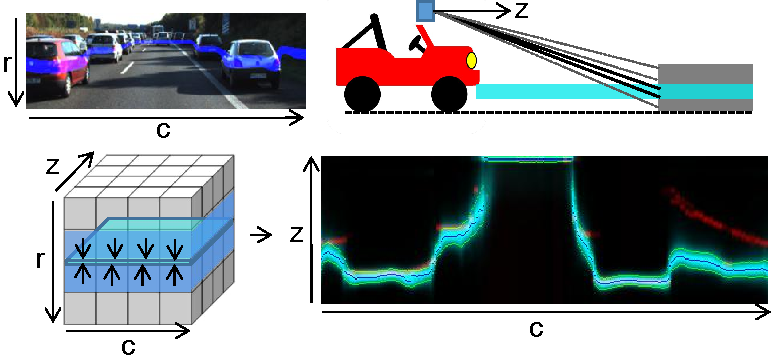
\includegraphics[width=1.0\textwidth]{figures/bev.pdf}
   \end{minipage}\hfill
   \centering
   \caption{Our state space consisting of a Depth Probability Volume (DPV) and Bird's Eye Uncertainty Field (UF)}
\end{figure}

\subsection{Curtain Planning}

With the Uncertainty Field (UF) extracted from the state space, we can use this to figure out where to place light curtains. We build upon prior work solving Light Curtain placement as a Constraint Optimization and Dynamic Programming problem \cite{Ancha_2020_ECCV}. A single light curtain placement is defined by a set of $T$ control points $\{\X_t\}_{t=1}^T$. We wish to maximize the objective $J(\X_1, \dots, \X_T) = \sum_{t=1}^T UF(\X_t)$ where $UF(\X)$ is the uncertaintiy field probabilies at the anchor location of $\X$.

The control points $\{\X_t\}_{t=1}^T$, where each $\X_t$ lies on the the camera ray $\R_t$, must be chosen to satisfy the physical constraints of the light curtain device: $|\theta(\X_{t+1}) - \theta(\X_t)| \leq \Delta \theta_\text{max}$ with $\theta_\text{max}$ being the maximum angular velocity of the Galvomirror. The problem is also discretized such that $\X_{t} \in \D\ $ and also lies along $\R_t$
\begin{align}
    &\arg \max_{\{\X_t\}_{t=1}^T} \sum_{t=1}^T UF(\X_t) \qquad \text{where}\ \X_t \in \D\ \nonumber\\
    &\text{subject to}\ |\theta(\X_{t+1}) - \theta(\X_t)| \leq \dtmax,\ \forall 1 \leq t < T
    \label{eq:constraint}
\end{align}

\begin{figure}[h]
   \centering
   \begin{minipage}{0.5\textwidth}
       \centering
       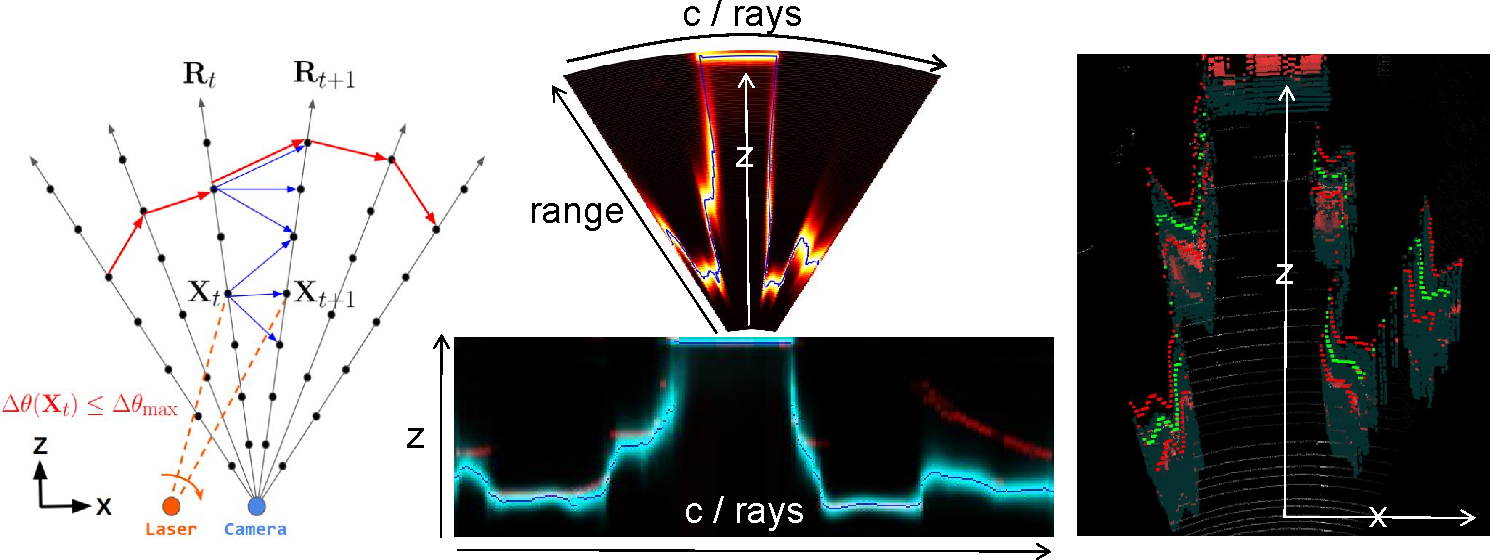
\includegraphics[width=1.0\textwidth]{figures/planner.pdf}
   \end{minipage}\hfill
   \centering
   \caption{\textbf{Left:} Light Curtain constraint graph subject to max angular velocity of Galvomirror. \textbf{Right:} Placing an optimal curtain along the highest probability region}
   \label{fig:plannerfig}
\end{figure}

\subsection{Curtain Placement}

The uncertainty field $UF$ contains the current uncertainty about piexl-wise object depths $\dd_{u, v}$ in the scene. Let us denote by $\pi(d^{c_k}\ |\ UF)$ the placement policy of the $k$-th light curtain, where $d^{c_k} = \{d^{c_k}_{u, v}\ |\ \forall u, v\}$. Our goal is to sample light curtain placements $d^{c_k} \sim \pi(d^{c_k}\ |\ UF)$ from this policy, and obtain intensities $i_{u, v}$ for every pixel.

To do this, we propose two policies $\pi_{0}$ and $\pi_{1}$. In Fig. ~\ref{fig:plannerfig}, we have placed a single curtain along the highest probability region per column of rays, but our goal is to maximize the information gained. To do this, we generate corresponding entropy fields $H(\X)_{i}$ to be fed to the planner from $UF(\X)$ based on two approaches: $\pi_{0}$ attempts to normalize each ray's distribution $UF(u)$ and warp the distribution such that a selected span from the mean is maximized. $\pi_{1}$ attempts to sample a point on the ray given $UF(u)$. The effects are seen in Fig. ~\ref{fig:m0m1}.

\begin{figure}[h]
   \centering
       \centering
       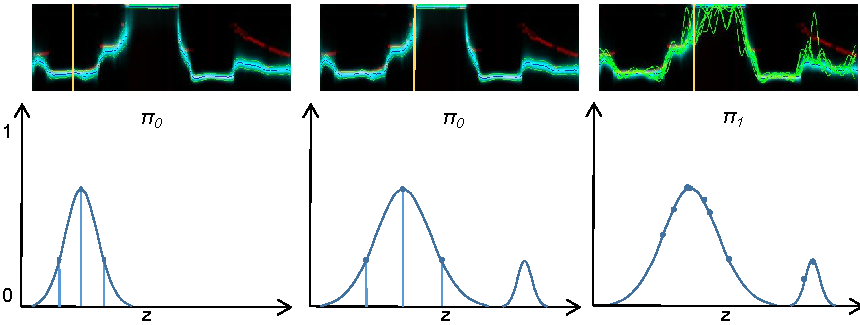
\includegraphics[width=0.48\textwidth]{figures/fields.pdf}
   \centering
   \caption{We look at where additional curtains are planned to be placed, given a depth distribution. \textbf{Left:} $\pi_{0}$ given a unimodal gaussian with small $\sigma$. \textbf{Middle:} $\pi_{0}$ given a multimodal gaussian with larger $\sigma$. \textbf{Right:} $\pi_{1}$ given a multimodal gaussian with larger $\sigma$. Observe that $\pi_{1}$ results in curtains being placed on the second mode.} 
   \label{fig:m0m1} 
\end{figure}

As seen in Fig. ~\ref{fig:m0m1}, strategy $\pi_{0}$ is able to generate fields that adaptively place additional curtains around a consistent span around the mean with some $\sigma_{\pi_{0}}$, but is unable to do so in cases of multimodal distributions. $\pi_{1}$ on the other hand is able to place a curtain around the 2nd modality, albeit with a lower probability. The inconsistency from ray to ray in $\pi_{1}$ however, may be impossible to image due to it exceeding the acceleration bounds, hence a spline fit is used with control points every 5 to 10 rays, resulting in an imagable but non-flat curtain placement. We see the effects of both in later experiments.

\subsection{Observation Model}

A curtain placement corresponds to specifying the depth for each camera ray indexed by $u$ from the top-down view. After placing the light curtain, intensities $i_{u,v}$ are imaged by the light curtain's camera at every pixel $(u, v)$. The produced intensity at each pixel is a function of the curtain placement depth $d^c_{u, v}$ on that camera ray, the unknown ground truth depth $\dd_{u, v}$ of that pixel, as well as the thickness of the light curtain $\sigma(u, v, d^c_{u, v})$ for a particular pixel and curtain placement. We use an approximate sensor model that describes the distribution of intensities. The intensity roughly decays exponentially as the distance between the light curtain placement $d^c_u$ and ground truth depth $\dd_{u, v}$ increases.  We also simulate sensor noise as a Gaussian distribution with standard deviation $\sigma_\text{noise}$. The overall sensor model $P(i_{u, v}\ |\ \dd_{u, v}, d^c_{u, v})$ can be described as:
\begin{align}
   &\nonumber P(i_{u, v}\ |\ \dd_{u, v}, d^c_{u, v}) \equiv\\
   &\quad \mathcal{N} \Big(i_{u, v}\ |\ \exp \Big(-\Bigg(\frac{d^c_{u, v} - \dd_{u, v}}{\sigma(u, v, d^c_{u, v})}\Bigg)^2\Big), \sigma_\text{noise}^2\Big)
   \label{eqn:sensor_model}
\end{align}

Note that when $d^c_{u, v} = \dd_{u, v}$, the mean intensity is $1$ (the maximum value), and it reduces exponentially as the light curtain is placed farther from the true surface.

\subsection{Recursive Bayesian Update}
\newcommand{\qb}{q'}
\newcommand{\before}[1]{{\color{blue} P_\text{prev}(u, v, #1)}}
\newcommand{\after}[1]{{\color{red} P_\text{next}(u, v, #1)}}

How do we incorporate the newly acquired information about the scene from the light curtain, to update our current beliefs of object depths? Since we have a probabilistic sensor model, we can use the Bayes' rule to infer the posterior distribution of the ground truth depths given the observations. Let $\before{q}$ denote the probability of the depth at pixel $(u, v)$ being equal to $d_q$ before sensing, and $\after{q}$ the updated probability after sensing. Then by Bayes' rule:
\begin{align*}
   &\after{q} \\
   &\hspace{5pt}= P(\dd_{u, v} = d_q\ |\ i_{u, v}, d^{c_k}_{u, v}) \\
   &\hspace{5pt}= \frac{P(\dd_{u, v} = d_q) \cdot P(i_{u, v}\ |\ \dd_{u, v} = d_q, d^{c_k}_{u, v})}{P(i_{u, v}\ |\ d^{c_k}_{u, v})}\\
   &\hspace{5pt}= \frac{P(\dd_{u, v} = d_q) \cdot P(i_{u, v}\ |\ \dd_{u, v} = d_q, d^{c_k}_{u, v})}{\sum_{\qb=0}^{N-1} P(\dd_{u, v} = d_{\qb}) \cdot P(i_{u, v}\ |\ \dd_{u, v} = d_{\qb}, d^{c_k}_{u, v})}\\
   &\hspace{5pt}= \frac{\before{q} \cdot P(i_{u, v}\ |\ \dd_{u, v} = d_q, d^{c_k}_{u, v})}{\sum_{\qb=0}^{N-1} \before{\qb} \cdot P(i_{u, v}\ |\ \dd_{u, v} = d_{\qb}, d^{c_k}_{u, v})}
\end{align*}

Note that $P(i_{u, v}\ |\ \dd_{u, v} = d_q, d^{c_k}_{u, v})$ is the sensor model whose form is given in Equation~\ref{eqn:sensor_model}.


% We now have returns from curtains $\mathbf{C}$ with each $\mathbf{C}_{i}$ containing $[x,y,z,i]$, the 3D position and intensity value in the same spatial resolution as $I$, planned based on a particular policy, conditioned on our prior distribution $P(\mathbf{d}_{t})$ at time $t$. We need to convert $\mathbf{C}_{i}$ into a likelihood distribution $P(\mathbf{c}_{t}|\mathbf{d}_{t})$, such that this Hidden Markov Model representation and sum of log likelihoods holds true:
% \small
% \begin{align}
%    P\left(\mathbf{d}_{0},...,\mathbf{d}_{T},\mathbf{c}_{1},...,\mathbf{c}_{T}\right)= 
%    P\left(\mathbf{d}_{0}\right)\mathbf{\mathbf{\prod}_{\mathrm{t=1}}^{\mathrm{T}}}P\left(\mathbf{c}_{t}|\mathbf{d}_{t}\right)P\left(\mathbf{d}_{t}|\mathbf{d}_{t-1}\right) \nonumber\\
%    \log\left(P\left(\mathbf{c}_{t}|\mathbf{d}_{t}\right)\right)=\stackrel[i=0]{n}{\sum}\left(\log\left(P\left(\mathbf{c_{\mathit{i}}}_{t}|\mathbf{d}_{t}\right)\right)\right)
%    \label{eq:hmm}
% \end{align}
% \normalsize

If we place $K$ light curtains at a given timestep, we can incorporate the information received from all of them into our Bayesian update simultaneously. Since the sensor noise is independent of curtain placement, the likelihoods of the observed intensities can be multiplied across the curtains. Hence, the overall update becomes: 
\begin{align*}
   &\after{q} \\
   &\hspace{5pt}= \frac{\before{q} \cdot \prod_{k=1}^K P(i_{u, v}\ |\ \dd_{u, v} = d_q, d^{c_k}_{u, v})}{\sum_{\qb=0}^{N-1} \before{\qb} \cdot \prod_{k=1}^K P(i_{u, v}\ |\ \dd_{u, v} = d_{\qb}, d^{c_k}_{u, v})}
\end{align*} 

\begin{figure}[h]
   \centering
   \begin{minipage}{0.5\textwidth}
       \centering
       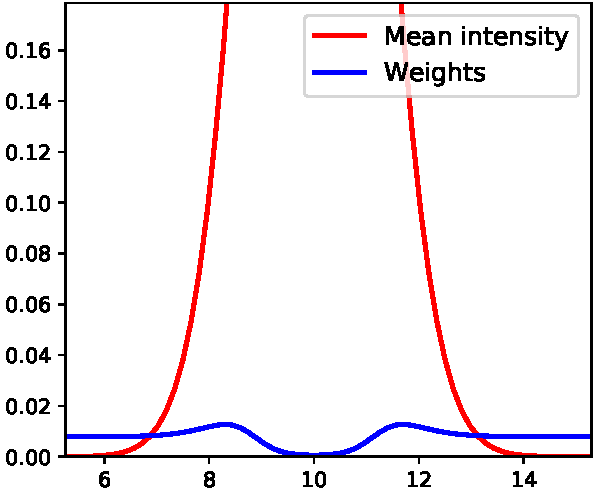
\includegraphics[width=0.31\textwidth]{figures/aa.pdf}
       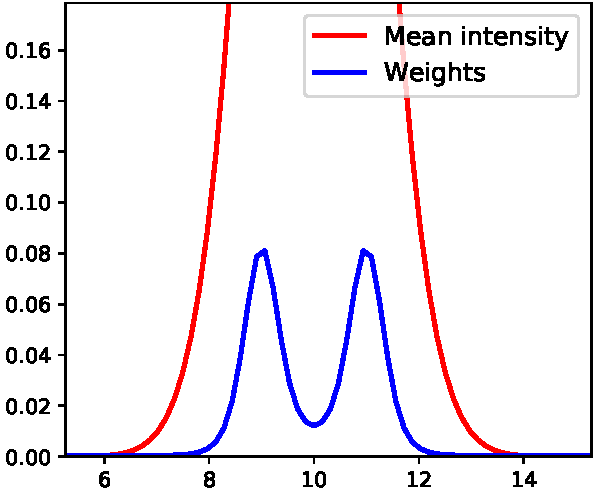
\includegraphics[width=0.31\textwidth]{figures/bb.pdf}
       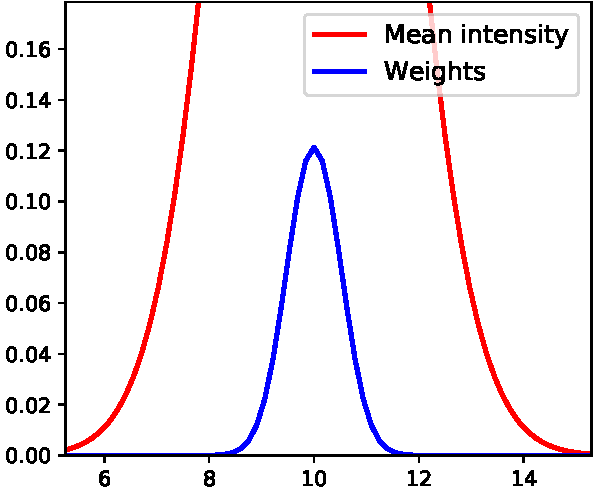
\includegraphics[width=0.31\textwidth]{figures/cc.pdf}
   \end{minipage}\hfill
   \centering
   \caption{Our sensor model produces a PDF where a low intensity leads to an inverted gaussian at the region of measurement, with other regions being uniform. Medium intensities mean the curtain isn't placed exactly on the object so is likely to be on either side, and consequently high intensities lead to the peak rising}
   \label{fig:updatemodel}
\end{figure}

The effects of this model as the placement depth $d^c_{u, v}$, curtain thickness $\sigma(u, v, d^c_{u, v})$ and intensity $i$ change is seen in Fig. ~\ref{fig:updatemodel}. One can observe that low intensities lead to an \textit{inverting gaussian} like PDF $P\left(\mathbf{d}_{u,v}^{c_{k}}\right)$ with other regions being uniform, indicating that it is somewhat certain that an object doesn't exist at that location, but is uniformly uncertain about the other unmeasured regions. A medium intensity indicates that the curtain may not exactly be on the surface, and so could be on either side of the measured location. Eventually as the intensity rises, so does the value of the peak.